\Section{MPEG Decoder in StreamIt}

% TODO: recalculate lines of code using statement count (num of ;)
We implemented an MPEG-2 decoder in StreamIt. It is a fully portable
implementation in that the application is not architecture
dependent. The implementation was carried out by one student
programmer with no prior understanding of MPEG. The development
spanned eight weeks from specification~\cite{mpeg-spec} to the first
fully functional MPEG decoder. The StreamIt code is nearly 4,921 lines
of code with 48 static streams. The MPEG stream parser is the largest
single filter, consisting of 1,924 lines of code.  The compiler
compiles the 48 static streams in the decoder into 2,150 filters for a
picture resolution of 352x240. In contrast, the reference C
implementation~\cite{reference-mpeg-c} is nearly 9,832 lines of code,
although it provides several features such as interlacing and
multi-layer streams that are not yet implemented in the StreamIt
decoder.

A noteworthy aspect of the StreamIt implementation is its
malleability. We illustrate this using two specific examples. 
In the first example, we focus on the video sampling rates. MPEG-2
streams are encoded using a 4:2:0 sampling rate, which achieve a 50\%
reduction in the number of bits required to represent a video, with
little noticeable loss of color. However, better quality is possible
with higher sampling rates since more color information is retained
from the original picture. In this paper, we'll describe how our
decoder implementation, originally designed to deal with 4:2:0
sampling rate is modified for a 4:2:2 sampling rate.

In the second example, we describe a straight forward language-level
transformation that exposes the data-parellism across macroblocks in a
picture. This is done in the context of the motion compensator. We
initially decribe the simplest implementation of the motion
compensator, which is a coarse grained filter operating at the
granularity of pictures. Then, we illustrate a more parallel
implementation that operates at finer granularity (i.e., macroblocks),
and show that the migration path is trivial.

\SubSection{Video Sampling Rate}

Macroblocks specify colors using a luminance channel to represent
saturation (color intensity), and two chrominance channels to
represent hue. The human eye is more sensitive to changes in
saturation than changes in hue, so the chrominance channels are
frequently compressed by downsampling the chrominance data within a
macroblock. The type of chrominance downsampling an MPEG-2 encoder
uses is its {\it chrominance format}. The most common chrominance
format is 4:2:0, which uses a single block for each of the chrominance
channels, downsampling each of the two channels from 16x16 to 8x8.  An
alternate chrominance format is 4:2:2. It uses two blocks for each
chrominance channel, downsampling each of the channels from 16x16 to
8x16. The possible chrominance formats are shown in
Figure~\ref{fig:chroma-format}.

To support the 4:2:2 chrominance format in our StreamIt decoder, we
modified 31 lines and added 20 new lines. Of the 31 modified lines, 23
were trivial modifications to pass a variable representing the
chrominance format as a stream parameter. The greatest substantial
change was to the decoding splitjoin previously illustrated in
Figure~\ref{fig:decoding-sj}. In the case of a 4:2:2 sampling rate,
the chrominance data, as it appears on the input tape, alternates
between each of the two chrominance channels. Thus, a a two-tiered
splitjoin is used to properly recover the appropriate chrominance
channels. The new splitjoin is shown in Figure~\ref{fig:chroma-format}.
\begin{figure*}[t]
 \begin{minipage}[t]{4.0in}
   {
    \begin{scriptsize}
    \begin{verbatim} 
    // N = macroblock size + motion vector data size;
    // W = picture width (resolution in pixels);
    // H = picture width (resolution in pixels);

    int->int splitjoin(int chromaFormat) {
      int xUpSample, yUpSample;

      if (chromaFormat == 420) { // 4:2:0 chroma format
        split roundrobin(4*N, 2*N);
        xUpSample = yUpSample = 2;
      } else {                   // 4:2:2 chroma format
        split roundrobin(4*N, 4*N);
        xUpSample = 2;
        yUpSample = 0;
      }

      add LuminanceChannel(W, H, 0, 0, chromaFormat);

      add int->int splitjoin {
        split roundrobin(N, N);
        add ChrominanceChannel(W, H, xUpsample, yUpSample, chromaFormat);
        add ChrominanceChannel(W, H, xUpsample, yupsample, chromaFormat);
        join roundrobin(1, 1);
      }

      join roundrobin(1, 2);
    }
    \end{verbatim}
    \end{scriptsize}
   }
   % \vspace{-3pt}
   \caption{Decoding stream to handle 4:2:0 and 4:2:2 chroma formats.}
   \label{fig:chroma-stream}
  \end{minipage}
  \begin{minipage}[t]{2.0in}
  {
   \begin{center}
    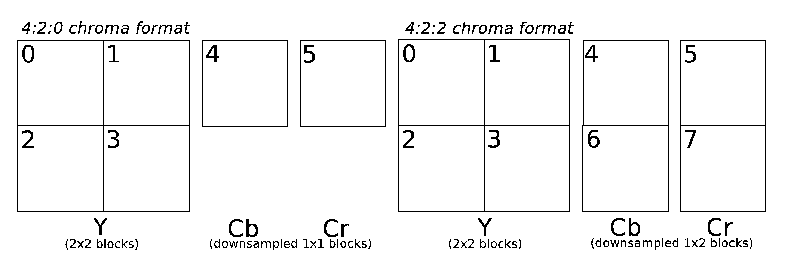
\epsfig{file=chroma_format.eps, width=3in}
    \caption{4:2:0 and 4:2:2 chrominance formats showing macroblock ordering}
    \label{fig:chroma-format}
   \end{center}
  }
  \end{minipage}
\end{figure*}





\SubSection{Motion Compensation}

An MPEG decoder accepts a bitstream as input and performs Huffman and
run-length decoding (VLD).  This process results in a set of
quantized, frequency-domain macroblocks and corresponding motion
vectors.  The decoder inverse quantizes (IQ) the macroblocks and then
performs an inverse DCT (IDCT) to convert the macroblocks to the
spatial domain.  For predictively coded macroblocks, the decoder
performs motion compensation (MC) using the motion vector to find a
corresponding macroblock in a previously decoded, stored reference
frame.  This reference macroblock is added to the current macroblock
to recover the original picture data.  If the current macroblock is
part of an I- or P-frame, then the decoder stores it for future
reference.  Figure~\ref{fig:dec_block} shows the block diagram of the
decode sequence.

\begin{figure}[htbp]
\centerline{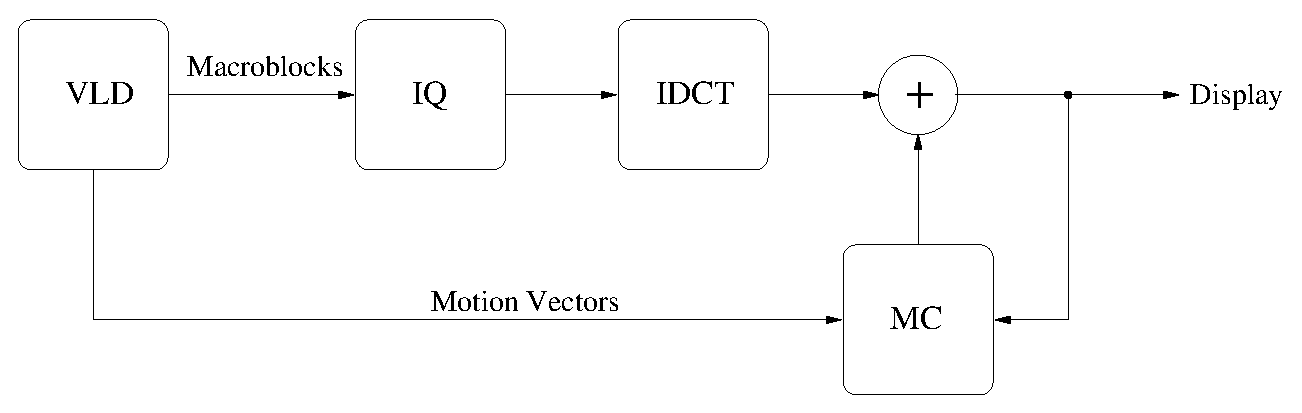
\epsfig{file=dec_block.eps,width=5in}}
\caption{Block diagram of MPEG-2 decode.}
\label{fig:dec_block}
\end{figure}

Our strategy for parallelizing MPEG-2 decoding is based on exploiting
data parallelism among macroblocks.  Using this scheme, the Huffman
and run-length decoding is inherently serial, as macroblock boundaries
can only be discovered by performing the decode operation.  Once this
decode is complete, a parallel implemenation can spread macroblocks
across independent processing elements (PEs) which can run
concurrently.  Each PE performs the inverse quantization, inverse
discrete cosine transform, and motion compensation.  Furthermore, each
PE locally stores reference macroblocks for future motion
compensation.  Using this strategy, PEs can execute independently with
one exception.

This exception occurs when a PE is performing motion compensation and
the corresponding motion vector indicates a reference macroblock
stored on a separate PE.  In this case, inter-PE communication occurs
to send the required reference data to the requesting PE.  This
situation is not uncommon, and it becomes more common as the number of
PEs increases for a fixed picture size.

One simple scheme for handling this situation is to have every PE
broadcast its decoded macroblocks to all other PEs.  This solution has
the benefit of being conceptualy easy to understand and implement.
However, broadcast communication can be very inefficient and it
generally does not scale well for large numbers of PEs.

A more sophisticated implementation takes advantage of algorithmic
knowledge to limit the amount of inter-PE communication.
Specifically, such an implementation exploits the fact
that MPEG-2 motion vectors have a bounded length.  Therefore, the
number of potential reference macroblocks for a predictively coded
macroblock is just a small subset of the total number of macroblocks.
This sophisticated implementation does not broadcast reference data to
all PEs, but sends data only to the PEs which might need it for
reference.  Furthermore, by ensuring that adjacent ranges of
macroblocks are allocated to adjacent PEs, this implementation ensures
that communication is kept local, as illustrated in
Figure~\ref{fig:mb_alloc}.  Such local communication patterns allow
such an implementation to scale much more efficiently as more PEs are
made available.

\begin{figure}[htbp]
\centerline{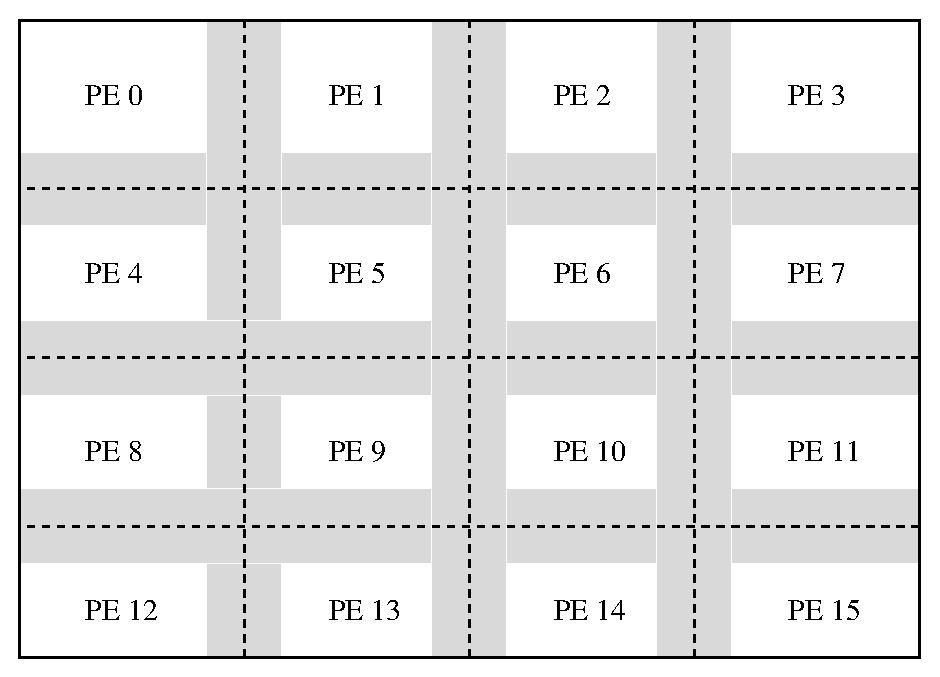
\epsfig{file=mb_alloc.eps,width=5in}}
\caption{Potential allocation of a reference frame among sixteen
processing elements.  Regions in gray represent reference macroblocks
that are communicated among neighboring processors.}
\label{fig:mb_alloc}
\end{figure}

The disadvantage of this latter implementation is that it can be quite
complicated to keep track of which PEs contain which macroblocks.
Furthermore, the local communication scheme can be more difficult to
schedule than a broadcast for some parallel processors.  However,
StreamIt provides mechanisms which allow programmers to expose these
local communication patterns to the compiler.  The compiler handles
the burden of allocating macroblocks to PEs and scheduling local
communication. The remainder of this section illustrates these
concepts in the context of MPEG-2 decoding.

\paragraph{Coarse-grained Implemenation}
\paragraph{Fine-grained Implemenation}
